\documentclass[preprint,12pt]{elsarticle}
\usepackage[utf8]{inputenc}
\usepackage[T1]{fontenc}
\usepackage{lmodern}
\usepackage{amsmath,amssymb}
\usepackage{booktabs}
\usepackage{graphicx}
\usepackage{multirow}
\usepackage{xurl}
\usepackage[hidelinks]{hyperref}
\usepackage{lineno}
\usepackage{framed}
\newenvironment{answer}[1]{\begin{framed}\noindent\textbf{#1.}\ }{\end{framed}}
\journal{Empirical Software Engineering}

\begin{document}
\begin{frontmatter}

\title{Memorised, Not Generated: Verbatim Recall of Published Fixtures in LLM-Generated Test Data, Measured Across Five Models and Eight Public Schemas}

\author{Vijay Prasad Javvadi\corref{cor1}}
\ead{vijay@vijayjavvadiresearch.ai}
\cortext[cor1]{Corresponding author. ORCID: 0009-0004-1192-6906.}
\address{Independent Researcher, Plainsboro, NJ, USA}

\begin{abstract}
Developers and LLM-based test generators now routinely ask a language model for the test data a test needs, and the model obliges with rows that look realistic. This paper asks whether that realism is generated or recalled, and answers with an executable measurement. We ask five models (Claude Sonnet 4.6 and 5.5, GPT-4o and GPT-5.6 Terra, and the open-weight Qwen3-235B) to emit test data for eight open-source database schemas that ship human-written fixtures, and compute a copy rate: the share of emitted rows whose high-cardinality text fields occur verbatim in the shipped fixture. On the three most widely mirrored schemas, Northwind, Chinook and Pagila, every model copies: Northwind at 23--76\,\% of rows exactly and up to 98\,\% within a small edit distance, Chinook at 2--35\,\%, Pagila at 4--37\,\%; the newer model of each vendor copies more than its predecessor. A plan-then-execute design, in which the model writes a generation plan for a constraint-aware engine, copies 0\,\% at a thirtieth of the token cost and the same validity. On Oracle's HR schema every model scores zero against the current fixture, because Oracle rewrote the data in 2021; against the 2015--2019 edition Claude Sonnet 5.5 reproduces the entire employees table verbatim and three other models reproduce 30--97\,\% of its text fields. A renamed-schema control, in which every identifier is replaced by a synonym, removes the distributional match to the fixtures ($p=0.016$) at unchanged validity ($p=1.0$) but not the row copying on Northwind, which one model recognises from its business description alone; the control is a lower bound, the copy rate the measurement. An exploratory downstream experiment with an LLM test generator finds no reliable change in mutation kills from provisioned fixtures. Every input is checksummed and every number is regenerated by released scripts.
\end{abstract}

\begin{keyword}
software testing \sep test data generation \sep memorisation \sep benchmark contamination \sep large language models \sep LLM-based test generation \sep empirical software engineering
\end{keyword}
\end{frontmatter}

\linenumbers

\section{Introduction}
\label{sec:intro}

A test needs data. A generated test for a service that lists orders exercises nothing unless orders exist; a fixture whose foreign keys point nowhere does not load. Developers now routinely ask a large language model (LLM) to produce test data for a schema, and the model usually obliges with rows that look plausible: company names that read like companies, product names that read like products. This paper asks one question about that practice, whether the plausibility is generated or recalled, and answers it with an executable measurement.

The schemas on which test-data tools are demonstrated and evaluated, Northwind, Sakila, Chinook and their relatives, have been mirrored in tutorials and repositories for two decades together with their sample data. A model that reproduces the sample data has not generated anything, and an evaluation that scores its output against that same data measures recall. We measure recall directly, as the memorisation literature does~\cite{carlini2023quantifying,riddell2024contamination}: a copy rate, the share of emitted rows whose free-text fields occur verbatim or near-verbatim in the shipped fixture. We compute it for five models from three vendors, including an open-weight model, on eight public schemas, and for one schema against three editions of its fixture, because the data a model recalls need not be the data that ships today. We complement the copy rate with a renamed-schema control, in which every table and column is replaced by a synonym and the dataset names are removed, and show what the control does and does not remove.

The mechanism matters because it suggests the remedy. Instead of emitting rows, the model can write a compact generation plan (which generator to use per column, which distributions, which references) that a deterministic engine executes in dependency order, so that keys, uniqueness and CHECK constraints are the engine's responsibility and the data never passes through the model. SynthData~\cite{synthdata}, the author's tool, implements this design; we use it as the instrument that makes the plan arm executable, not as the object of the study, and compare it with the most favourable direct-emission harness we could build, on the same schemas, scoring every emitted row by inserting it into PostgreSQL with all constraints enabled. The comparison answers a second, narrower question: what it costs, in validity and tokens, to obtain test data by a route that cannot copy.

A third, exploratory experiment asks whether any of this matters to an LLM test generator. We take a pipeline with an executable mutation benchmark from our earlier work (manuscript under review)~\cite{javvadi2026raitg}, pre-load its database-backed services with the generated fixtures, and measure usable-test yield and mutation kills. The experiment turned out to be underpowered for the kill-rate question, and we report it as exploratory, with the one mechanism it did identify.

\paragraph{Findings} Verbatim recall of published fixtures is general across models and grows with model generation. On Northwind, Chinook and Pagila all five models copy rows: Claude Sonnet 5.5 reproduces 76\,\% of the Northwind rows exactly and 98\,\% within a small edit distance, GPT-5.6 55\,\%, the open-weight Qwen3-235B 36\,\%, and each vendor's newer model copies more than its predecessor. On Oracle's HR schema the copy rate against the current fixture is zero for every model because the data was rewritten in 2021, and against the 2015--2019 edition Claude Sonnet 5.5 reproduces all 107 employee rows in every column; a copy rate measured against the fixture that ships today is therefore a lower bound. The plan arm and Faker copy nothing. The renamed-schema control removes the distributional match of emitted data to the fixtures (categorical distance 0.25 to 0.73, $p=0.016$) while validity does not move ($p=1.0$), which is consistent with recall and not with a harder schema, but it does not remove the copying on Northwind, which one model recognises from its domain description alone. Plan-then-execute and direct emission reach the same validity at 500 rows per table, the plan arm at a thirtieth of the token cost and with zero copying. Downstream, provisioned fixtures do not change what an LLM test generator detects, at a sensitivity of 6--12 mutants, and lower its usable yield because generated tests assume an empty database; stating the database state in the prompt restores the yield.

\paragraph{Contributions}
(i) A copy-rate measurement of LLM-generated relational data against the fixtures that ship with public schemas, applied to five models and eight schemas, with the finding that verbatim recall is general, grows with model generation, and can be invisible against a revised fixture (Section~\ref{sec:rq1}).
(ii) A renamed-schema control for the same data, and the measurement of what it removes (the distributional match) and what it does not (domain-cued copying), so that the control is used as a lower bound and paired with the copy rate (Section~\ref{sec:e1b}).
(iii) An executable benchmark of the plan-then-execute alternative against the same fixtures, with a PostgreSQL scorer that classifies every rejected row, showing that a route that cannot copy reaches the same validity at a thirtieth of the cost (Section~\ref{sec:rq2}).
(iv) An exploratory downstream experiment, reported with its sensitivity, in which constraint-valid fixtures do not change an LLM test generator's mutation kills and lower its usable yield through an identified fixture-contract mechanism (Section~\ref{sec:rq3}).

\section{Background}
\label{sec:background}

\subsection{Direct emission}
The model receives the DDL, a description of the business domain and a row target, and answers with rows. A single response cannot hold thousands of rows, so the harness requests rows in chunks, table by table in foreign-key order, and shows the model a sample of the parent keys it has already emitted so that references can be valid. This is the naive approach in its most favourable form: the model is told everything it needs to satisfy every constraint. Cost scales with the number of rows, and every row's constraints are the model's to satisfy.

\subsection{Plan-then-execute}
SynthData\footnote{\texttt{@vijaypjavvadi/synthdata}, MIT licence. The study freezes version 1.2.2; file checksums are in the artifact.} parses the DDL into tables, columns, types, primary and foreign keys, UNIQUE and CHECK constraints (including \texttt{IN} lists and enum types). It asks the model once for a YAML plan: one generator per column from a fixed vocabulary (\texttt{sequence}, \texttt{fk}, \texttt{choice} with weights, \texttt{int}, \texttt{float} and \texttt{lognormal} ranges, \texttt{date} and \texttt{datetime} ranges, \texttt{template}, \texttt{faker} methods, \texttt{expr}), with per-table row counts and a seed. It then executes the plan deterministically: tables in dependency order, foreign keys sampled from keys that exist (self-references are supported, subject to defect \#8, Section~\ref{sec:rq2}), uniqueness enforced over single and composite key sets, CHECK constraints enforced. Four profiles are available: \texttt{functional} (happy-path rows), \texttt{edge} (CHECK endpoints, maximum-length strings, NULLs in nullable columns, every enum value), \texttt{negative} (rows that each violate exactly one constraint, tagged with the violation) and \texttt{volume}. An \texttt{auto} mode infers a plan from the DDL with no LLM at all. Cost is one LLM call regardless of row count; the model controls distributions only through the plan vocabulary.

Fig.~\ref{fig:arms} contrasts the two designs: where the model stops, where the engine starts, and what each is asked to get right.

\begin{figure}[t]
\centering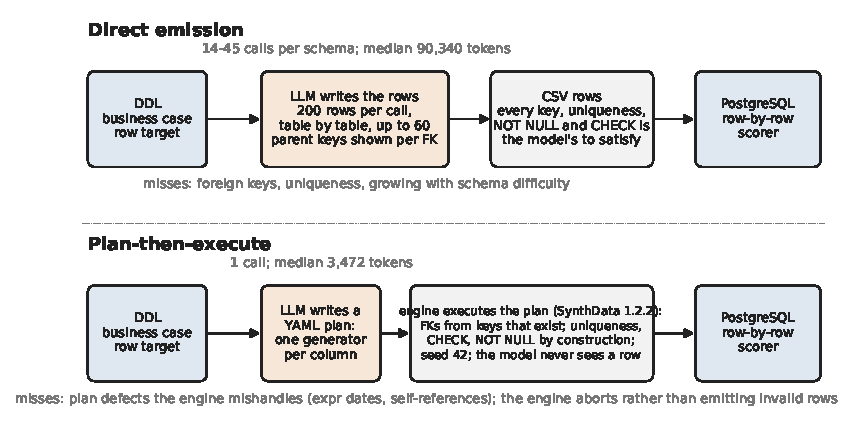
\includegraphics[width=\textwidth]{figures/fig0b_arms}
\caption{Direct emission versus plan-then-execute. In direct emission the model writes every row and every constraint is the model's to satisfy; in plan-then-execute the model writes one generation plan and a deterministic engine writes the rows, so keys, uniqueness, CHECK and NOT NULL hold by construction and the model's mistakes surface as plan defects. Token medians per schema cell are from E1 (Section~\ref{sec:cost}).}
\label{fig:arms}
\end{figure}

\subsection{The author's position}
SynthData is the author's tool, and the study uses it as an instrument: the plan arm exists so that the copy rate of a route that cannot copy can be measured beside the route that can. The study therefore gives every arm identical inputs (the same DDL, the same frozen business case, the same row targets, the same seeds) and scores every arm with the same database and scorer. The tool version was frozen before any measured run (version 1.2.2, published to npm on 11 September 2026 at 18:01 UTC and checksummed in the artifact). Defects that the study found afterwards were fixed in the next release, 1.2.3, published the same day, but no measured cell uses it; they are listed in Section~\ref{sec:rq2} and in the artifact. Section~\ref{sec:threats} returns to the conflict of interest.

\section{Study design}
\label{sec:method}
Fig.~\ref{fig:overview} gives the study in one view: a main experiment with its control and its extension (E1, E1b, E1c), each pairing LLM arms with non-LLM and human references and each scored by an executable oracle, and an exploratory downstream experiment (E2).

\begin{figure}[t]
\centering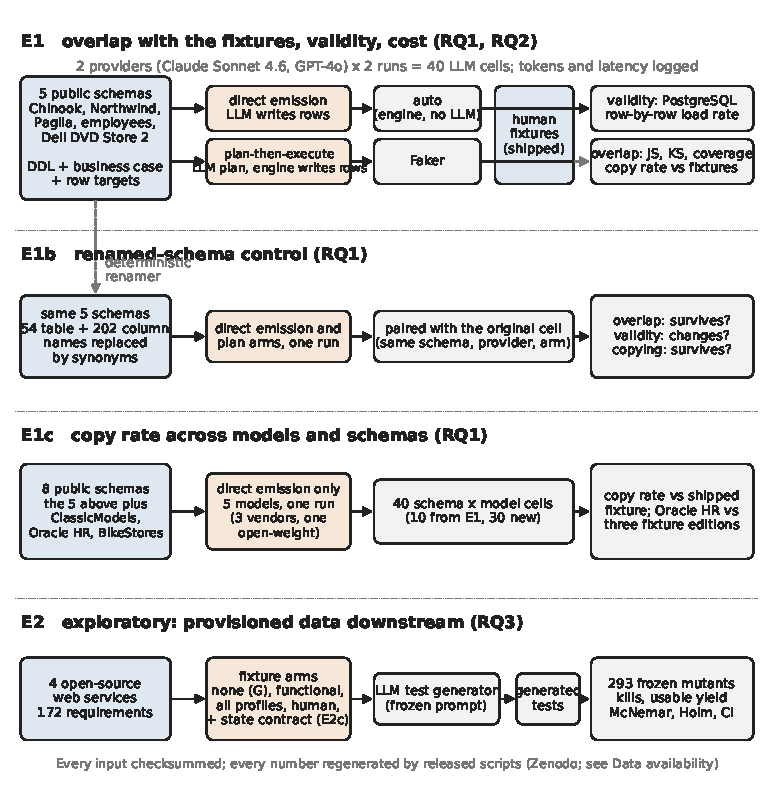
\includegraphics[width=\textwidth]{figures/fig0_overview}
\caption{Study overview. E1 scores four generation arms and the shipped fixtures on five public schemas for overlap with the fixtures (distances and a copy rate), validity (PostgreSQL load rate) and cost; E1b reruns the LLM arms with every identifier renamed and pairs each cell with its original; E1c runs the direct arm with five models on eight schemas and computes the copy rate for every cell; E2, exploratory, feeds the E1 fixtures to an existing LLM test generator on four web services and scores the generated tests against 293 frozen mutants.}
\label{fig:overview}
\end{figure}

\subsection{Research questions}
\begin{description}
\item[RQ1 (memorisation)] What fraction of the rows an LLM emits for a public schema are verbatim copies of the fixture that ships with it; does the fraction depend on the model, the schema and the edition of the fixture; and how much of the emitted data's resemblance to the fixture survives when the schema's identifiers are renamed?
\item[RQ2 (the alternative route)] Does plan-then-execute, in which the data never passes through the model, satisfy the schema's declared constraints as reliably as direct emission, and at what cost?
\item[RQ3 (downstream, exploratory)] Given the same LLM test generator, does provisioning constraint-valid fixtures change the usable-test yield or the executable mutation kill rate, compared with letting the generator invent its own data?
\end{description}
RQ1 is answered by experiment E1 (overlap with the fixtures and copy rate, two models), its control E1b and its extension E1c (five models, eight schemas, three fixture editions); RQ2 by E1 (validity and cost); RQ3 by E2. Every LLM arm of E1, E1b and E2 runs on two model families, Claude Sonnet~4.6 and GPT-4o, so that no finding rests on one vendor; E1c adds the current model of each vendor and an open-weight model.



\subsection{Subjects}
Table~\ref{tab:subjects} lists the eight schemas with their declared constraints; the first five are the E1 subjects and the last three were added for E1c; the constraint surface is dominated by keys and nullability, with one CHECK and one UNIQUE clause across the five (Section~\ref{sec:threats} returns to this). Each ships human-written sample data under an open licence and loads into PostgreSQL~16 with constraints enabled. Their shapes differ. Pagila (film rental) has 15 base tables after collapsing the payment partitions, 18 foreign keys, an enum type and many-to-many bridges. Chinook (music store) has a self-referencing employee hierarchy and a composite-key bridge. Northwind (trading) has a self-reference, a composite primary key and two empty tables. \texttt{employees} (HR history) has 3.9~million rows, a CHECK constraint, a UNIQUE text column and date-range assignments. Dell DVD Store~2 (retail) has wide customer rows and no declared foreign keys between \texttt{orders}, \texttt{orderlines} and \texttt{products}. Pagila, Chinook and Northwind are widely mirrored with their sample data; \texttt{employees} is distributed with its data as a MySQL test database; Dell DVD Store~2 ships a generator rather than a fixed dataset and is the least likely of the five to have been seen with its rows. We do not know the providers' training sets, which is why the control in Section~\ref{sec:e1bdesign} exists. The three E1c schemas were chosen for the same property with less exposure to the LLM literature: ClassicModels (a scale-model retailer; the MySQL tutorial sample database, loaded from a mirrored dump), Oracle's HR schema (the sample schema of the Oracle documentation, loaded from Oracle's own repository), and BikeStores (a bicycle retailer; the SQL Server tutorial sample database, loaded from a mirrored copy of the vendor scripts). The HR fixture has been revised: Oracle rewrote names, phone numbers, e-mails and dates in schema version 21 (2021) and again by version 23, and the edition published from 2015 to 2019 is the 11g edition with every date shifted by sixteen years; we loaded the 2019 edition from the repository's history as well, which Section~\ref{sec:editions} uses. All eight were pinned to a commit or tag and their files checksummed before any generation; the Postgres ports of the three E1c schemas, with every type and constraint mapping, are in the artifact.

\begin{table}[t]
\centering\footnotesize\setlength{\tabcolsep}{4pt}
\caption{Subjects: the five E1 schemas and the three added in E1c. Constraint counts are declared clauses in the canonical DDL (NOT NULL counts columns, including key columns; Pagila's CHECK is the rating enum rewritten as \texttt{CHECK IN}). Human rows are the shipped fixture counts; row targets for the generated arms are $\min(\text{human}, 500)$ per table.}
\label{tab:subjects}
\resizebox{\textwidth}{!}{%
\begin{tabular}{llrrrrrrrl}
\toprule
Schema & Pinned source & Tables & Columns & PK & FK & UNIQUE & CHECK & NOT NULL & Human rows \\
\midrule
Pagila & pagila v3.1.0 & 15 & 86 & 15 & 18 & 0 & 1 & 71 & 46,273 \\
Chinook & chinook-database 7f67772 & 11 & 64 & 11 & 11 & 0 & 0 & 30 & 15,607 \\
Northwind & northwind\_psql cd0ef28 & 14 & 92 & 14 & 13 & 0 & 0 & 31 & 3,362 \\
employees & test\_db e324b56 & 6 & 24 & 6 & 6 & 1 & 1 & 23 & 3,919,015 \\
Dell DVD Store 2 & postgresDBSamples 2bdc953 & 8 & 52 & 5 & 3 & 0 & 0 & 39 & 172,716 \\
\midrule
ClassicModels & mysqlsampledatabase (bklogic 241750c) & 8 & 59 & 8 & 8 & 0 & 0 & 46 & 3,864 \\
Oracle HR & db-sample-schemas 6660bad (v23.3) & 7 & 35 & 7 & 9 & 1 & 2 & 17 & 216 \\
BikeStores & sqlservertutorial (ant-analytics mirror) & 9 & 52 & 9 & 11 & 1 & 0 & 36 & 9,071 \\
\bottomrule
\end{tabular}}
\end{table}

\paragraph{Canonical DDL} Each schema was exported from the PostgreSQL catalogue into one canonical file with inline PK, FK, UNIQUE, CHECK and NOT NULL clauses, enum types rewritten as \texttt{CHECK (col IN (\ldots))}, partitions collapsed and one non-portable column (Pagila's \texttt{tsvector}) dropped. Reloading the human fixtures into the canonical schema gives identical row counts and zero rejections on all eight. One deviation is recorded: the HR schema's departments--employees cycle is cut by omitting the manager foreign key of \texttt{departments}, because a canonical file has one self-contained \texttt{CREATE TABLE} per table.

\paragraph{Business cases} One text per schema, written from the project's public documentation only (never from the fixture data) and frozen with an MD5 before any run. Every arm receives the same case verbatim, plus the same row-target line.

\paragraph{Row targets} $\min(\text{human count}, 500)$ per table, chosen after timing the direct arm at roughly 100 seconds per 100 rows. The cap is conservative against the plan arm: the direct arm's dominant failure, repeated keys across chunks, grows with the number of rows, so a higher cap would widen the validity gap in the engine's favour. Overlap metrics compare a 500-row sample with the full human distribution.

\subsection{Arms for E1}
\begin{enumerate}
\item \textbf{Direct emission.} The model receives the canonical DDL, the business case, the table to fill, its exact row target, a sample of up to 60 already-emitted parent keys per foreign-key column, and the last 30 keys it emitted for the same table; it must answer with CSV only. Chunks of 200 rows; temperature 0; every call's tokens and latency are logged.
\item \textbf{Plan-then-execute.} SynthData's own system prompt and user-message format, temperature 0, one call; the plan is executed with seed 42 under the \texttt{functional} profile. The \texttt{edge} and \texttt{negative} profiles are executed from the run-1 plans without further LLM calls.
\item \textbf{Auto.} SynthData's no-LLM mode, seed 42.
\item \textbf{Faker.} A plain Faker~\cite{faker} script per schema with no referential resolution: what a developer gets from the ecosystem default.
\item \textbf{Human.} The shipped fixtures, unmodified.
\end{enumerate}
LLM arms run on both providers with two independent runs each: 40 LLM cells in total.

\subsection{Scoring validity}
\label{sec:scorer}
For each cell, a fresh database is created from the canonical DDL and the emitted CSVs are inserted row by row in foreign-key order inside a PL/pgSQL loop that catches every exception and records the table, row and SQLSTATE. Rows that violate anything are rejected, so a rejected parent makes its children fail their foreign key, which is the real cost of an invalid row. A retry pass re-attempts rows rejected only for foreign-key reasons until no progress is made, so that within-table order (a self-referencing hierarchy emitted child-before-parent) is never counted against an arm. Casts use base types so that declared lengths and precisions are enforced by the insert. SQLSTATE classes 23503, 23505, 23514, 23502 and 22xxx are reported as FK, UNIQUE, CHECK, NOT NULL and type/length. The scorer was validated on the human fixtures (100\,\% load on all five schemas) and on a Chinook copy with one planted violation of each class, which reports exactly the five planted rows plus their foreign-key cascade.

\subsection{Scoring overlap with the fixtures}
\label{sec:fidmetrics}
Per column, against the human fixture of the same schema. Categorical columns are of two kinds. \emph{Declared-domain} columns are enum, CHECK-IN and boolean columns, whose legal values are in the DDL. \emph{Free-text} columns are text columns with at most 30 distinct human values, such as city or job title, whose values are not in the DDL. For both we compute the Jensen--Shannon distance (base~2; 0 identical, 1 disjoint) and the fraction of human values present. Numeric and date columns get the two-sample Kolmogorov--Smirnov statistic and the fraction of the human range covered; foreign-key columns the absolute difference in fan-out Gini; nullable columns the null-rate difference. Aggregates are medians over a schema's columns; surrogate keys are excluded. We call this family of metrics \emph{overlap with the fixture} rather than fidelity or realism, and the split matters for RQ1: an arm can match a declared domain by reading the DDL and a numeric range by reading the business case, but it can match the distribution of a free-text column only by knowing the data, so on free-text columns a low distance is evidence of recall before it is evidence of realism. The copy rate of Section~\ref{sec:copy} is the row-level form of the same measurement.

\subsection{E1b: the renamed-schema control}
\label{sec:e1bdesign}
A deterministic renamer replaces every table and column identifier (54 table names and 202 distinct column names) with a synonym (\texttt{customer}$\to$\texttt{client}, \texttt{order}$\to$\texttt{purchase}, \texttt{film}$\to$\texttt{movie}, \texttt{us\_states}$\to$\texttt{state\_codes}, and so on), removes the dataset names and documentation references from the business cases, and applies the same synonyms to the case prose. Types, constraints, CHECK value lists, row targets, prompts and seeds are unchanged; the human fixtures reload into the renamed DDLs at 100\,\%, and the engine's \texttt{auto} mode reaches 100\,\% on all five. The LLM arms are rerun once per provider (20 cells) and each renamed cell is paired with the run-1 cell of the same schema, provider and arm. Two references calibrate the effect: the run-to-run variation of the original schemas (run 1 versus run 2) bounds what a rerun alone can change, and the least-mirrored schema (Dell DVD Store~2) bounds what renaming costs a model that has nothing to recall.

\subsection{E1c: more models, more schemas, more editions}
\label{sec:e1cdesign}
E1c extends the copy-rate measurement along the three axes on which the E1 result could be an artefact: the model, the schema and the fixture. It runs the direct arm only, with the E1 harness unchanged (same system prompt, 200-row chunks, parent-key context, seeds, row targets), on the eight schemas of Table~\ref{tab:subjects} with five models: the two E1 models, a then-current model of each commercial vendor (Claude Sonnet~5.5, released on 28 September 2026, and GPT-5.6 Terra, the mid-priced tier of the GPT-5.6 family released on 9 July 2026, chosen as the counterpart of the Sonnet tier; the flagship Sol tier was not run), and an open-weight model, Qwen3-235B-A22B-Instruct-2507 (Alibaba, July 2025), served through OpenRouter. The identifiers in Section~\ref{sec:reporting} are the strings the APIs accepted and, where the response carries one, echoed back. The E1 cells on the five E1 schemas are reused; the other 30 schema--model cells are new, one run each, 50 cells in all when the E1 second runs are counted. Two of the new models differ from the E1 setting in ways the API imposed and the logs record: both reject the temperature setting (Anthropic reports it as deprecated for the model, OpenAI accepts only the default), and Claude Sonnet~5.5 reasons before answering by default, which we could not switch off with the field we tried; the two therefore ran at the model defaults that a practitioner obtains out of the box, and a repeat of one cell (Oracle HR, Sonnet~5.5) shows the consequence, the copy rate moving between runs where the E1 models, at temperature 0, repeated within a point. OpenRouter routed the open-weight model to several hosts; the serving host of every call is logged. For Oracle HR the copy rate is computed against three fixture editions: the current one (v23.3), the 2015--2019 edition from the repository's history, and that edition with dates shifted back sixteen years, which reconstructs the 11g edition that the repository does not hold.

\subsection{E2: provisioned data downstream (exploratory)}
\label{sec:e2design}
E2 reuses the RAITG pipeline of~\cite{javvadi2026raitg}, whose requirements, mutants, harness and baseline run logs are archived on Zenodo as RAITG v5.0.0, with its scoring protocol unchanged. The pipeline covers 172 requirements over four community Python services (httpbin, fastapi-restful, flaskr, fastapi-task-manager). Tests are generated per requirement with the grounded prompt (SUT source injected, verification and repair on), extracted into per-service pytest harnesses, and filtered to \emph{known-good} units, those that pass on clean source. The known-good units are scored against 293 frozen mutants; a kill is a new failure or collection error. Three services have a database; httpbin has none and serves as a negative control.

For the three database-backed services we derived a DDL (flaskr's \texttt{schema.sql}; the SQLAlchemy \texttt{Task} model; the \texttt{players} table of the shipped SQLite file), wrote a business case from each project's README and REST examples, and generated fixtures with SynthData~1.2.2 (Claude plan, seed 42, three profiles). Each fixture was validated through the application itself: logins succeed and list endpoints return the fixture. The RAITG prompt (v1.5.0) gains one optional element, a \texttt{[TEST DATA]} block; without it the prompt is byte-identical to the published v1.4.0. Four arms:
\begin{description}
\item[G] the grounded arm of~\cite{javvadi2026raitg} (baseline). For Claude these are the archived run logs re-scored under the E2 harness; for GPT-4o they are new runs, since no archived GPT-4o logs exist.
\item[G+D-func] the functional fixture shown to the model and pre-loaded into the service's database at scoring.
\item[G+D-all] the same pre-loaded fixture, plus the \texttt{edge} rows shown as valid boundary payloads and the \texttt{negative} rows shown as invalid payloads with their violation tags. The database state is identical to G+D-func, so the difference isolates the information given to the model.
\item[G+D-human] the project's own fixture shown (flaskr's two users and one post; the 26 shipped players; the task manager ships none).
\item[G+D-state] added after the first four arms were scored (E2c): the G+D-func block followed by an explicit database-state contract, stating that the tables are never empty, that ids $1..N$ are taken, that the first row a test creates receives id $N+1$, that count assertions must be relative to $N$, that the listed rows are the ones to use for existing-row tests, and (for fastapi-restful) that squad numbers 1--26 are taken. The database state at scoring is identical to G+D-func; only the information given to the model differs. Run once, for Claude, against the run-1 baseline.
\end{description}
At scoring time, each arm's conftest provisions its fixture wherever the database is initialised: the default instance database, the harness fixtures, and any database a generated test creates itself through the application's \texttt{init\_db()} or \texttt{Base.metadata.create\_all()}. The promise made in the prompt therefore holds in the run. Two harness issues found during scoring, and the re-scoring of every arm under one corrected harness, are recorded in \ref{app:harness}. Two providers, two runs each for the first four arms. The hypothesis, written in the research plan on 11 September 2026 before any E2 run (the plan is in the artifact), was that the data block raises usable yield on the database-backed services and leaves httpbin unchanged, with any kill-rate gain concentrated on validation-path mutants. The E2c arm was designed after that hypothesis had been rejected, and its own expectations were written down before it ran (also in the artifact): that the state contract returns usable yield to the baseline level (aggregate $\ge 88$\,\%, task manager $\ge 90$\,\%), that the kill count stays within ten of the baseline, and that httpbin moves by at most seven.

\subsection{Statistics}
\label{sec:stats}
E1 and E1b comparisons are paired over cells (E1: schema $\times$ provider $\times$ run; E1b: renamed versus original per cell) and reported as the paired median difference with a bootstrap 95\,\% confidence interval (10,000 resamples, seed 42), Cliff's delta, and the Wilcoxon signed-rank $p$-value. Cells that share a schema are not independent, so we also report the schema-level result ($n=5$) as a sensitivity check. The copy-rate comparison (Section~\ref{sec:copy}) uses the same paired design over the ten renamed-versus-original direct-emission pairs, with the exact Wilcoxon test on the non-tied pairs. E1c is descriptive: it reports the copy rate per schema--model cell and counts the cells, per model and per schema, in which it exceeds one per cent; with one run per new cell and no planned contrast, no inferential statistic is attached to it. E2 comparisons are paired over mutants (the 293 per-mutant kill vectors of an arm versus its baseline in the same provider and run) with the exact McNemar test, a bootstrap 95\,\% confidence interval of the difference (1,000 resamples of mutants, seed 42), and a Holm correction over the twelve tests. Runs are reported side by side, never pooled.

\subsection{Reporting}
\label{sec:reporting}
We follow the guidelines for empirical studies involving LLMs of Baltes et al.~\cite{baltes2026guidelines,wagner2025towards}, which apply in full to a benchmarking study of this kind. Model versions and dates: \texttt{claude-sonnet-4-6} and \texttt{gpt-4o} as served by the providers' APIs on 11--12 September 2026 (E1, E1b, E2) and 22 September 2026 (E2c); for E1c, the same two plus \texttt{claude-sonnet-5-5}, \texttt{gpt-5.6-terra} and \texttt{qwen/qwen3-235b-a22b-2507} (via OpenRouter, serving host logged per call) on 4--5 October 2026, all recorded per call in the artifact's logs. The OpenAI and OpenRouter responses echo the served model, and the logs record \texttt{gpt-4o-2024-08-06} behind the \texttt{gpt-4o} alias and the two other identifiers unchanged; the Anthropic identifiers carry no date suffix and are the strings the API accepted. The artifact's \texttt{model\_identity\_check.py} re-queries each provider's model listing and a one-token completion for every identifier and stores the result beside the logs. Temperature 0 throughout E1, E1b and E2, with the caveat that temperature 0 is not determinism (Section~\ref{sec:threats}); the two newest commercial models in E1c reject the setting and ran at their defaults, reasoning included (Section~\ref{sec:e1cdesign}). Every raw output is archived. Architecture: API calls through the arm scripts named in Section~\ref{sec:method}, no retrieval, no agents, no fine-tuning (Fig.~\ref{fig:overview}). Prompts: every prompt, static and dynamic, is in the artifact verbatim, with the prompt version that E2 froze (\texttt{v1.5.0}, and \texttt{v1.5.1} for E2c). Repetitions: two independent runs per LLM cell in E1 and E2, reported side by side, and one run per new E1c cell, declared as such; the minimum detectable effect this affords in E2 is stated in Section~\ref{sec:stats}, and the E2c arm is a single run declared as such. Metrics: validity is database acceptance, overlap with the fixtures is a battery of column-wise distances plus a copy rate, downstream effect is mutation kills on frozen mutants; each is justified where it is introduced rather than by prior use. Baselines: a no-LLM engine mode and Faker for E1, the generator's own unaided output and the human fixture for E2. Open-weight model: Qwen3-235B in E1c, on every schema; E1, E1b and E2 use commercial models only. Contamination: the renamed-schema control and the copy rate are the study's treatment of it. Cost: tokens, calls and wall time per cell (Table~\ref{tab:cost}). Human validation: none is needed, since every oracle is executable. Data availability: Section~\ref{sec:data}.

\section{RQ1: memorisation}
\label{sec:rq1}

\subsection{Overlap with the fixtures before the control}
\label{sec:fidelity}
On the surface, direct emission overlaps the human data far more than plan-then-execute does. Over the 18 paired cells in which both arms produced data, the median categorical Jensen--Shannon distance is 0.083 for direct emission and 1.000 for the plan arm ($p=0.003$, Cliff's $\delta=0.51$); the fraction of human categorical values reproduced is 1.00 versus 0.00 ($p=0.004$). Numeric and date distributions do not differ (KS 0.522 versus 0.501, $p=0.83$); plans cover the human numeric ranges better (0.960 versus 0.520, $p=0.019$); emitted rows imitate the human foreign-key fan-out slightly better (Gini difference 0.068 versus 0.101, $p=0.028$).

Splitting the categorical columns changes the picture. On declared-domain columns, which exist only in Pagila among the five schemas (the rating enum and two booleans; four cells), both arms match the human distributions: median JS 0.043 for the plan arm and 0.110 for direct emission. The entire categorical gap is in free-text columns (median 1.000 versus 0.083, identical to the aggregate). Two further observations point the same way. With Claude, the direct arm scores a JS distance of exactly 0.000 on 22 of the 36 categorical columns of Northwind and on 8 of the 11 of Pagila, in both runs (median 0.000): on those columns it re-emits the published dataset value for value. And on Dell DVD Store~2, the schema least likely to have been seen with its data, the direct arm's JS distance (0.41 with Claude, 0.88 with GPT-4o) and value coverage (0.88, 0.22) are no better than the plan arm's (0.47, 0.86 and 0.60, 0.19).

\subsection{The renamed-schema control}
\label{sec:e1b}
Table~\ref{tab:e1b} and Fig.~\ref{fig:e1b} pair each renamed direct-emission cell with its original run-1 cell.

\begin{table}[t]
\centering\footnotesize
\caption{E1b: direct-emission cells, original versus renamed schema (run 1). Load rate in \%; JS = median categorical Jensen--Shannon distance to the human data; cov = fraction of human categorical values reproduced; $\Delta$JS = renamed $-$ original.}
\label{tab:e1b}
\resizebox{\textwidth}{!}{%
\begin{tabular}{llccccccc}
\toprule
Schema & Provider & load orig & load ren & JS orig & JS ren & $\Delta$JS & cov orig & cov ren \\
\midrule
Chinook & Claude & 93.8 & 99.2 & 0.000 & 0.326 & $+0.33$ & 1.00 & 0.80 \\
Chinook & GPT-4o & 99.7 & 99.7 & 1.000 & 1.000 & $0.00$ & 0.00 & 0.00 \\
Northwind & Claude & 98.4 & 97.2 & 0.000 & 0.263 & $+0.26$ & 1.00 & 0.95 \\
Northwind & GPT-4o & 77.3 & 87.8 & 0.587 & 1.000 & $+0.41$ & 0.63 & 0.00 \\
Pagila & Claude & 99.9 & 99.6 & 0.000 & 1.000 & $+1.00$ & 1.00 & 0.00 \\
Pagila & GPT-4o & 94.7 & 96.1 & 1.000 & 1.000 & $0.00$ & 0.00 & 0.00 \\
employees & Claude & 99.8 & 95.4 & 0.054 & 0.085 & $+0.03$ & 1.00 & 1.00 \\
employees & GPT-4o & 98.6 & 98.7 & 0.083 & 0.389 & $+0.31$ & 1.00 & 1.00 \\
Dell DVD Store 2 & Claude & 100 & 97.7 & 0.406 & 0.589 & $+0.18$ & 0.88 & 0.83 \\
Dell DVD Store 2 & GPT-4o & 100 & 100 & 0.875 & 0.875 & $0.00$ & 0.22 & 0.22 \\
\midrule
median & & 99.2 & 98.2 & 0.245 & 0.732 & $+0.22$ & 0.94 & 0.51 \\
\bottomrule
\end{tabular}}
\end{table}

\begin{figure}[t]
\centering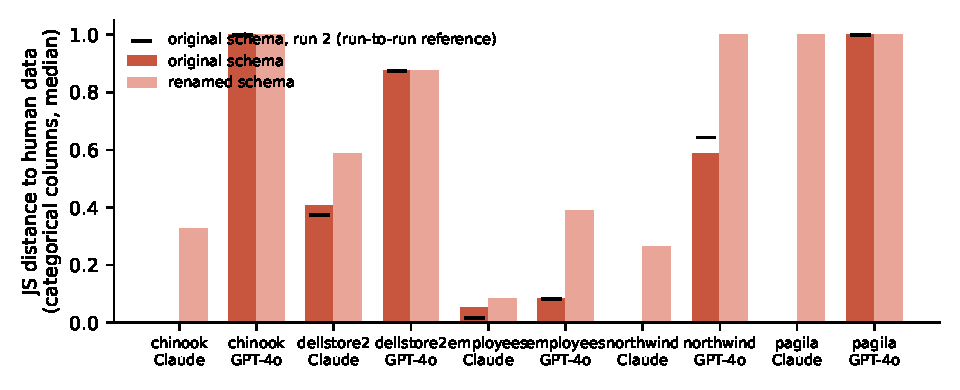
\includegraphics[width=\textwidth]{figures/fig3_e1b_memorisation}
\caption{E1b: categorical distance of directly emitted data to the human fixtures, original versus renamed identifiers (direct arm, run 1). The black tick on each original bar is the same cell's run-2 value, i.e.\ the run-to-run reference (median $|\Delta|$ 0.000, maximum 0.056). Claude's exact reproduction of the categorical distributions of Northwind, Chinook and Pagila disappears when the names change (its row-level copying does not, on Northwind: Table~\ref{tab:copy}); Dell DVD Store~2, the least-mirrored schema, moves by 0.18 (Claude) and 0.00 (GPT-4o).}
\label{fig:e1b}
\end{figure}

\paragraph{Validity is unaffected} Direct-emission load rates do not change under renaming (median 99.2\,\% versus 98.2\,\%; paired median difference 0.000, 95\,\% CI $[-0.012, +0.028]$; $p=1.0$). The models' ability to satisfy constraints does not depend on recognising the dataset, which also rules out the alternative reading that the renamed schemas are simply harder to understand.

\paragraph{The overlap does not survive} The direct arm's median categorical JS distance rises from 0.245 to 0.732 (paired median difference $+0.22$, 95\,\% CI $[0.00, +0.36]$; $p=0.016$), its value coverage falls from 0.94 to 0.51 ($p=0.062$), and its numeric/date KS statistic rises from 0.522 to 0.602 (median difference $+0.06$, CI $[0.00, +0.09]$; $p=0.023$). Two references put these deltas in scale. The run-to-run variation of the same metric on the original schemas (run 1 versus run 2, ten schema--provider pairs) has median 0.000 and maximum 0.056, so a rerun alone does not move the distance. And on Dell DVD Store~2, the least-mirrored schema, renaming costs Claude 0.18 and GPT-4o 0.00, which bounds what synonyms cost a model with nothing to recall. On the three widely mirrored schemas Claude's deltas are $+0.33$ (Chinook), $+0.26$ (Northwind) and $+1.00$ (Pagila), and GPT-4o, which was already at JS~1.0 on Chinook and Pagila, moves $+0.41$ on Northwind, the one it had partly reproduced. Claude's exact reproduction of Pagila (JS 0.000, coverage 1.0) becomes a disjoint distribution (JS 1.000, coverage 0.0).

This pattern is consistent with recall and not with the renamed schemas being harder: the effect is far above run-to-run noise and above the renaming cost on the unfamiliar schema, it appears where the published data is famous and the model had reproduced it exactly, and validity does not move. On ten pairs the interval touches zero, so the control alone would be weak evidence; it is the direct measurement of the next two subsections that carries the claim. Under renamed schemas the direct arm's categorical overlap (median 0.73) is much closer to the plan arm's (median 1.0) than the 0.08-versus-1.00 comparison of Section~\ref{sec:fidelity} suggested. On a schema the model does not recognise, neither approach reproduces the categorical distributions of the human data; the plan arm covers numeric ranges better and the direct arm imitates fan-out slightly better. The large categorical overlap of direct emission on public schemas is where recall of Northwind, Sakila and Chinook would show, and the next subsection measures that recall directly.

\subsection{Verbatim reproduction}
\label{sec:copy}
A distributional distance shows that the direct arm matches the human data; it does not show that it copies rows. The memorisation literature quantifies memorisation as a copy rate, the fraction of outputs that reproduce training text exactly or within a small edit distance~\cite{carlini2023quantifying,riddell2024contamination}, so we add one. For every emitted row we take its values in the schema's high-cardinality text columns (columns with more than thirty distinct human values: names, titles, addresses, descriptions) and ask whether the same tuple occurs in the shipped fixture. Keys and low-cardinality columns are excluded: a key carries no content, and a low-cardinality column (a country, a genre) is already scored by the JS distance and can be matched by knowing the domain rather than the data. We report the exact-match rate pooled over the schema's rows and a near-match rate at a normalised Indel similarity of at least 0.9, and put the plan arm and Faker beside them as floors. Numbers, booleans and dates are normalised before comparison. For the two schemas whose fixtures exceed 50,000 rows per table (employees, Dell DVD Store~2) the human side is the first 50,000 rows, so their rates are lower bounds. The script and the per-table results are in the artifact.

\begin{table}[t]
\centering\small
\caption{Verbatim reproduction: share of directly emitted rows whose high-cardinality text fields occur in the shipped fixture, exact and at Indel similarity $\geq 0.9$; original schema (runs 1 and 2) versus renamed schema (run 1). Plan arm and Faker on the original schema as floors; ``--'' = the plan cell aborted (defect \#6).}
\label{tab:copy}
\begin{tabular}{llrrrrrrr}
\toprule
Schema & Provider & \multicolumn{3}{c}{Exact (\%)} & \multicolumn{2}{c}{$\geq$0.9 (\%)} & Plan & Faker \\
\cmidrule(lr){3-5}\cmidrule(lr){6-7}
 & & orig.\ r1 & orig.\ r2 & renamed & orig. & renamed & (\%) & (\%) \\
\midrule
Northwind & Claude & 53.5 & 57.9 & 63.7 & 96.6 & 89.2 & 0.0 & 0.0 \\
 & GPT-4o & 22.8 & 25.5 & 6.3 & 31.4 & 6.3 & -- &  \\
Chinook & Claude & 35.1 & 34.0 & 19.7 & 45.0 & 27.6 & 0.0 & 0.1 \\
 & GPT-4o & 1.6 & 1.8 & 1.8 & 1.8 & 1.8 & 0.0 &  \\
Pagila & Claude & 14.8 & 14.4 & 5.6 & 16.0 & 6.1 & 3.3 & 0.0 \\
 & GPT-4o & 4.4 & 4.4 & 5.1 & 4.5 & 5.1 & 2.9 &  \\
employees & Claude & 20.4 & 50.6 & 0.0 & 21.8 & 0.6 & 0.0 & 0.0 \\
 & GPT-4o & 0.0 & 0.0 & 0.0 & 0.8 & 0.4 & 0.0 &  \\
Dell DVD Store~2 & Claude & 0.0 & 0.0 & 0.0 & 0.0 & 0.0 & 0.0 & 0.0 \\
 & GPT-4o & 0.0 & 0.0 & 0.0 & 0.0 & 0.0 & 0.0 &  \\
\bottomrule
\end{tabular}
\end{table}

Table~\ref{tab:copy} gives the result. The floors are at zero: Faker copies no rows, and the plan arm's only non-zero cells are Pagila's 3\,\%, where a plan emits real country names. On the original schemas, Claude's direct arm reproduces 53.5\,\% of the Northwind rows verbatim and 96.6\,\% within similarity 0.9: the products table begins with Chai, Chang and Aniseed Syrup in the fixture's order, and the customers and suppliers are the fixture's companies. It reproduces 35.1\,\% of Chinook (artists, albums, customers) and 14.8\,\% of Pagila (the 200 actors at 99.5\,\%, the 109 countries at 84\,\%, none of the film descriptions), at least 20.4\,\% of employees, and none of Dell DVD Store~2, whose shipped data is randomly generated and has nothing to recall. GPT-4o copies 22.8\,\% of Northwind and little else. Run 2 reproduces run 1 within 0.4 percentage points on every cell except employees (50.6\,\% versus 20.4\,\%), where the copied rows are name pairs drawn from the dataset's small name lists.

Renaming removes the copying where it was cued by the identifiers and not where it was not. The Claude copy rate falls to zero on employees, to 5.6\,\% on Pagila and to 19.7\,\% on Chinook, and GPT-4o's Northwind rate falls from 22.8\,\% to 6.3\,\%. Claude's Northwind rate does not fall: 63.7\,\% exact and 89.2\,\% within 0.9, with the renamed \texttt{items} table still listing Chai, Chang, Aniseed Syrup and Chef Anton's Cajun Seasoning. The renamed business case, which the control keeps, describes ``a specialty-foods import/export trading company'' whose items belong to eight named sections (beverages, condiments, confections, and so on); that description identifies Northwind without a single identifier, and Claude recalls the dataset from it. Over the ten pairs the paired difference is therefore not significant (median 0.000, 95\,\% CI $[-0.155, +0.004]$; Wilcoxon $p=0.30$ over the seven non-tied pairs). The pairs fall into three groups: schemas with nothing to recall, which stay at zero; schemas whose recall is name-cued, where renaming removes or halves it; and one schema recalled from its domain description, where renaming changes nothing.

Two conclusions follow. First, much of the overlap that direct emission shows on the mirrored schemas is copying in the plain sense: between a seventh and a half of the rows Claude emits are the fixture's rows. Second, the renamed-schema control under-states memorisation rather than over-stating it. What renaming removes is the categorical-distribution match of Table~\ref{tab:e1b}; the residual copy rate on Northwind shows that renaming identifiers while keeping a recognisable domain description does not make a famous schema unseen, and an overlap or realism result on a public schema should be read against a copy rate, not only against a control.

One further cue survives renaming. Claude's renamed-Pagila plan still placed rental dates in 2005--2006, the Sakila era, so structural recognition is not fully removed by identifier renaming either. The control removes lexical identity, not structure or domain; a stronger control would perturb values and rewrite the business case as well, or use a schema published after the providers' training cut-offs.

\paragraph{The plan arm under renaming} Plan-arm load falls from a mean of 0.888 (run 1) to 0.711, and every sub-100 renamed cell is again defect \#6 or \#7 (the engine-defects paragraph of Section~\ref{sec:rq2}): with synonym names both models reached for \texttt{expr} date arithmetic in 4 of 10 plans (3 of 20 in E1), and the engine handles it wrongly. The plan arm's validity ceiling is set by the engine's handling of LLM-written plans, not by the model.

\subsection{Across models and schemas (E1c)}
\label{sec:models}
Table~\ref{tab:copymodels} gives the copy rate of the direct arm for the eight schemas and five models of E1c, one run per cell; the E1 cells are the run-1 values of Table~\ref{tab:copy}. Three things are general. First, the three widely mirrored schemas are copied by every model: Northwind by all five (22.8--76.0\,\% of rows exact, 31--98\,\% within similarity 0.9), Chinook by all five (1.6--35.1\,\%), Pagila by all five (4.4--37.1\,\%). The open-weight Qwen3-235B copies Northwind at 35.9\,\% and its \texttt{us\_states} and \texttt{customers} tables at 98\,\% and 64\,\%, so the effect is not a property of one vendor's training data. Second, the newer model of each vendor copies more than its predecessor on every E1 schema: Claude Sonnet~5.5 against 4.6 on Northwind 76.0 against 53.5, on Pagila 37.1 against 14.8, on employees 40.8 against 20.4; GPT-5.6 against GPT-4o on Northwind 54.8 against 22.8, on Pagila 22.1 against 4.4, on Chinook 11.1 against 1.6. Whatever the cause (larger models, more training data, more epochs over the same tutorials), the copy rate measured in E1 on 2024--2026 models is a lower bound for their successors, not a peak. Third, the two schemas with nothing to recall stay at zero for every model: Dell DVD Store~2, whose shipped data is generated, and Oracle HR, for the reason the next subsection gives. The two new schemas with hand-written fixtures separate the Claude models from the rest: ClassicModels is copied by Sonnet~4.6 (14.9\,\%; its \texttt{customers} table at 33\,\% exact and 76\,\% near) and Sonnet~5.5 (10.1\,\%) and by no other model, and BikeStores by Sonnet~5.5 alone (11.8\,\%; its \texttt{products} table at 30\,\% exact and 72\,\% near). Over the 40 cells, 20 have a copy rate above one per cent: 5 of 8 schemas for Sonnet~4.6, 6 of 8 for Sonnet~5.5, and 3 of 8 for each of GPT-4o, GPT-5.6 and Qwen3-235B.

\begin{table}[t]
\centering\small
\caption{E1c: copy rate of the direct arm by schema and model, one run per cell (the E1 models on the E1 schemas are their run-1 cells). Exact (\%) is the share of emitted rows whose high-cardinality text fields occur verbatim in the shipped fixture; in parentheses, the share within normalised Indel similarity $\geq 0.9$. Oracle HR is scored against the current fixture here; see Table~\ref{tab:editions}.}
\label{tab:copymodels}
\setlength{\tabcolsep}{4pt}
\begin{tabular}{lrrrrr}
\toprule
Schema & Sonnet 4.6 & Sonnet 5.5 & GPT-4o & GPT-5.6 Terra & Qwen3-235B \\
\midrule
Northwind & 53.5 (96.6) & 76.0 (98.3) & 22.8 (31.4) & 54.8 (86.8) & 35.9 (61.5) \\
Chinook & 35.1 (45.0) & 34.3 (38.7) & 1.6 (1.8) & 11.1 (11.1) & 7.3 (9.7) \\
Pagila & 14.8 (16.0) & 37.1 (38.6) & 4.4 (4.5) & 22.1 (22.6) & 10.1 (10.5) \\
employees & 20.4 (21.8) & 40.8 (41.0) & 0.0 (0.8) & 0.0 (0.4) & 0.0 (0.0) \\
Dell DVD Store 2 & 0.0 (0.0) & 0.0 (0.2) & 0.0 (0.0) & 0.0 (0.0) & 0.0 (0.0) \\
ClassicModels & 14.9 (21.7) & 10.1 (17.1) & 0.0 (0.0) & 0.0 (0.0) & 0.1 (0.6) \\
Oracle HR (current) & 0.0 (0.0) & 0.0 (0.0) & 0.0 (0.0) & 0.0 (0.0) & 0.0 (0.0) \\
BikeStores & 0.0 (3.9) & 11.8 (28.1) & 0.0 (0.0) & 0.0 (7.4) & 0.0 (0.0) \\
\bottomrule
\end{tabular}
\end{table}

\subsection{Which edition is recalled (Oracle HR)}
\label{sec:editions}
Against the fixture that ships today, every model's copy rate on Oracle HR is zero, and the overlap metric tells a different story: 59--66\,\% of the distinct text values that four of the five models emit for the \texttt{employees} table occur in the fixture. The rows are not copies because the fixture changed. Oracle revised the HR data in schema version 21 (2021), changing some surnames, every phone number and e-mail, and every date, and the edition published from 2015 to 2019 is itself the 11g edition with all dates shifted by sixteen years. Table~\ref{tab:editions} scores the same emitted rows against the three editions. Claude Sonnet~5.5 reproduces the 2019 edition of the 107-row \texttt{employees} table in full: every row, every column, including the phone numbers and the salaries. Claude Sonnet~4.6 reproduces 97\,\% of its text fields with the hire dates of the 11g edition, that is, the edition that circulated in tutorials for the longest. GPT-5.6 reproduces 30\,\% and Qwen3-235B 36\,\% of the text fields, with a quarter to a third of complete rows; GPT-4o reproduces nothing. The first row of the table, the president, is emitted by four of the five models with the name, e-mail alias, phone number, job code and salary of the 2015--2019 edition; only the hire date (Sonnet~4.6 gives the 11g date) and one missing department column (Qwen) differ, and GPT-4o invents a different person.

\begin{table}[t]
\centering\small
\caption{Oracle HR, \texttt{employees} table (107 rows): copy rate of the same emitted rows against three editions of the fixture. Text = exact match of the high-cardinality text fields (\%); all = exact match of every content column (\%); near = text fields within similarity $\geq 0.9$ (\%). The 11g edition is the 2015--2019 edition with dates shifted back sixteen years.}
\label{tab:editions}
\begin{tabular}{lrrrrr}
\toprule
 & current (v23) & \multicolumn{3}{c}{2015--2019 edition} & 11g \\
\cmidrule(lr){3-5}
Model & text & text & all & near & all \\
\midrule
Claude Sonnet 4.6 & 0.0 & 97.2 & 0.0 & 99.1 & 4.7 \\
Claude Sonnet 5.5 & 0.0 & 100.0 & 100.0 & 100.0 & 0.0 \\
GPT-4o & 0.0 & 0.0 & 0.0 & 0.0 & 0.0 \\
GPT-5.6 Terra & 0.0 & 29.9 & 26.2 & 64.5 & 0.0 \\
Qwen3-235B & 0.0 & 35.5 & 29.9 & 40.2 & 0.0 \\
\bottomrule
\end{tabular}
\end{table}

The consequence for measurement is the point. A copy rate, or any overlap metric, computed against the fixture that ships today is a lower bound on recall whenever the fixture has been revised, and the sample databases that models have read most have been revised: Northwind has a dozen ports, Sakila and Pagila differ, and HR has three editions. A zero against the current fixture, as on Dell DVD Store~2, means nothing to recall only when no earlier edition exists to check. Where one exists, the copy rate should be computed against each, and the highest reported.


\begin{answer}{Answer to RQ1}
Verbatim recall of published fixtures by LLM-emitted test data is general. All five models copy the three most-mirrored schemas (Northwind at 23--76\,\% of rows exact, up to 98\,\% near), the newer model of each vendor copies more than its predecessor, the open-weight model copies as the commercial ones do, and the plan arm and Faker copy nothing. On Oracle HR the copy rate against the current fixture is zero because the fixture was rewritten; against the 2015--2019 edition Claude Sonnet~5.5 reproduces the employees table in full. The renamed-schema control removes the distributional overlap, which is consistent with recall, but not the copying cued by a recognisable domain description; it is a lower bound, and the copy rate, computed against every edition of the fixture, is the measurement to report.
\end{answer}

\section{RQ2: the route that cannot copy}
\label{sec:rq2}

\subsection{Validity}
Table~\ref{tab:e1load} and Fig.~\ref{fig:e1load} give the load rate of every cell. Over the 20 paired (schema, provider, run) cells the plan arm's mean is 0.886 with median 1.000 and the direct arm's mean is 0.962 with median 0.987. The two engine aborts (defect \#6, Northwind with GPT-4o, both runs), counted as zero, put the direct arm ahead on the mean by 0.076; on the paired median difference the arms are level ($+0.004$, 95\,\% CI $[-0.017, +0.015]$; Wilcoxon $p=0.85$; schema-level $p=0.81$). Excluding the two aborts ($n=18$) the means are 0.985 and 0.983 and the plan arm is marginally ahead (paired median difference $+0.006$, CI $[+0.002, +0.017]$; Cliff's $\delta=0.53$; $p=0.29$). We state the result as: at 500 rows per table on these schemas, plan-then-execute has no validity advantage over direct emission, and a user who counts the aborts sees it slightly behind. The difference between the arms is in how they fail.

\begin{table}[t]
\centering\footnotesize\setlength{\tabcolsep}{3.5pt}
\caption{E1 load rate (\% of emitted rows accepted by PostgreSQL with all constraints on), run 1 / run 2. ``abort'' = the engine aborted on the LLM-written plan (defect \#6) and produced no data, counted as 0.}
\label{tab:e1load}
\resizebox{\textwidth}{!}{%
\begin{tabular}{lcccccccc}
\toprule
& \multicolumn{2}{c}{plan-then-execute} & \multicolumn{2}{c}{direct emission} & auto & Faker & human \\
\cmidrule(lr){2-3}\cmidrule(lr){4-5}
Schema & Claude & GPT-4o & Claude & GPT-4o & (no LLM) & & \\
\midrule
Chinook   & 100 / 100 & 100 / 100 & 93.8 / 98.1 & 99.7 / 99.6 & 100 & 99.3 & 100 \\
Northwind & 100 / 100 & abort / abort & 98.4 / 97.7 & 77.3 / 77.1 & 100 & 23.5 & 100 \\
Dell DVD Store 2 & 93.8 / 100 & 93.9 / 93.8 & 99.97 / 98.8 & 100 / 99.97 & 100 & 100 & 100 \\
Pagila    & 100 / 100 & 100 / 90.8 & 99.9 / 99.6 & 94.7 / 94.4 & 100 & 52.3 & 100 \\
employees & 100 / 100 & 100 / 100 & 99.8 / 99.3 & 98.6 / 97.7 & 100 & 0.4 & 100 \\
\bottomrule
\end{tabular}}
\end{table}

\begin{figure}[t]
\centering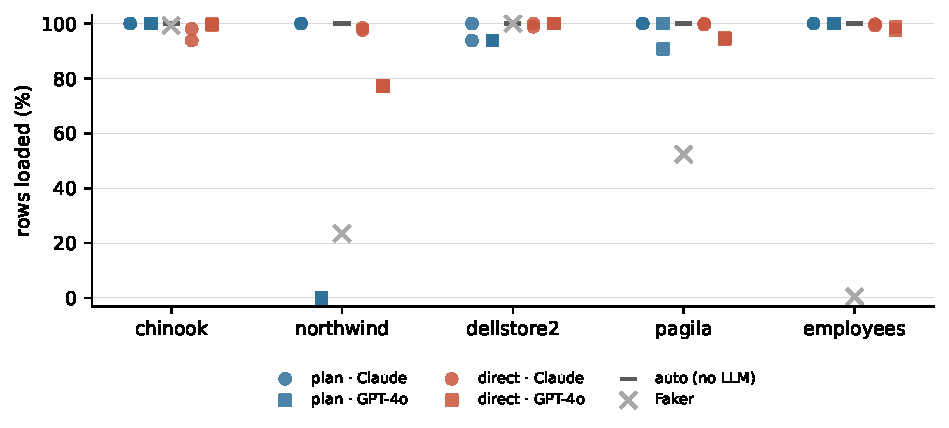
\includegraphics[width=\textwidth]{figures/fig1_e1_load}
\caption{E1 load rate per schema and arm (both providers, both runs). The plan arm is at 100\,\% except where an engine defect bites; direct emission degrades with schema difficulty and model.}
\label{fig:e1load}
\end{figure}

The plan arm is bimodal: 14 of the 18 executed cells load at exactly 100\,\%, and each of the remaining four is attributable to one engine defect visible in the plan and the rejection log. Three Dell DVD Store~2 cells lose 185--187 rows to duplicate primary keys because the model wrote \texttt{\{gen: fk, ref: inventory.prod\_id\}} for a primary-key column and the engine sampled the reference with replacement (defect \#7; the schema declares no foreign key there, which is why the model reached for one). One Pagila cell loses 443 rows because an \texttt{expr} generator received its date operand as a string and concatenated instead of adding (\texttt{2025-03-18 16:25:007}; defect \#6), and the two Northwind GPT-4o cells abort on the same defect. Across all executed plan cells the engine emitted zero foreign-key, CHECK and NOT NULL violations; its 559 UNIQUE and 443 type rejections are the two defects.

Direct emission is never 100\,\% on a schema with declared foreign keys (its one 100\,\% is Dell DVD Store~2, which declares none), and its rejections are the model's: 504 foreign-key, 1,009 uniqueness, 4 NOT NULL and 79 type/length violations over 20 cells. The effect grows with schema difficulty and shrinks with model strength: on Northwind, GPT-4o loads 77.3 and 77.1\,\% in the two runs (152/139 foreign-key, 147/164 uniqueness and 13/12 type rejections), Claude 98.4 and 97.7\,\%. Repeated keys across chunks are the dominant failure: the model is told the last 30 keys it emitted and still repeats keys from earlier chunks.

\paragraph{Engine defects} An executable study against a tool finds defects in the tool, and they are results. Five defects were found and fixed before the study version was frozen at 1.2.2 (numeric precision, composite primary keys, small UNIQUE value pools, \texttt{varchar(n)} enforcement, and \texttt{fk} on a column without a declared foreign key; the v1.1.0 smoke numbers that motivated them are in the artifact). Four were found afterwards by LLM-written plans and are not fixed in the study version: \#6, \texttt{expr} receives dates as strings (seven cells across E1 and E1b); \#7, \texttt{fk} on a primary-key column samples with replacement (Dell DVD Store~2); \#8, a self-referencing \texttt{fk} on a NOT NULL column emits NULL for the first rows (found while validating the E2 fixtures); \#9, the YAML parser rejects a multi-line flow sequence that PyYAML accepts (the E2 task-manager plan). Every plan-arm miss in E1 and E1b is \#6 or \#7; the plan arm's validity ceiling is the engine's plan handling, and a user of version 1.2.2 inherits these defects. \#6 and \#7 were fixed in 1.2.3, published after the freeze; no number in this paper was re-run on it.

The baselines frame the result. The engine's no-LLM \texttt{auto} mode loads 100\,\% on all five schemas. Validity, on these schemas, comes from the engine; the LLM's contribution to the plan arm is the plan's semantics, which Section~\ref{sec:rq1} measures as overlap with the fixtures and as copy rate. The Faker script, the ecosystem default, loads 100\,\% only where every foreign key happens to point at a table whose keys are $1\ldots N$ (Dell DVD Store~2, Chinook) and collapses elsewhere (Northwind 23.5\,\%, Pagila 52.3\,\%, \texttt{employees} 0.4\,\%): the referential engine is what a Faker script lacks. The plan arm's copy rate is zero on every schema (Table~\ref{tab:copy}): a plan names generators and distributions, not values, so the route cannot reproduce a fixture even where the model that wrote the plan has memorised it.



\subsection{Cost}
\label{sec:cost}
Per cell (Fig.~\ref{fig:e1tokens}), the plan arm uses a median of 3,472 tokens in one call and the direct arm 90,340 tokens in 14--45 calls; the median of the per-cell ratios is 29.5 (the ratio of the medians is 26.0). Wall-time medians are 15\,s and 658\,s (per-cell median ratio 46; the longest direct cell, Pagila with Claude, took 28 minutes). Over the study the plan arm consumed 40k input and 31k output tokens, the direct arm 865k and 1,441k. Table~\ref{tab:cost} gives the per-cell medians and ranges by provider; we report tokens and wall time rather than money because list prices change, and the artifact logs every call so that a reader can price the study at any date. The direct arm's spread is wide (a factor of four in tokens across schemas) because cost scales with the row count; the plan arm's is narrow because a plan's length depends on the number of columns, not rows.

\begin{table}[t]
\centering\small
\caption{E1 cost per schema cell by arm and provider: median (min--max) over the ten cells, and study totals. Wall time is the sum of call latencies.}
\label{tab:cost}
\begin{tabular}{llrrrrr}
\toprule
Arm & Provider & Cells & Calls & Input tokens & Output tokens & Wall time (s) \\
\midrule
Plan-then-execute & Claude & 10 & 1 (1--1) & 2,191 (1,684--2,668) & 1,548 (741--3,082) & 22 (9--39) \\
 & GPT-4o & 10 & 1 (1--1) & 1,831 (1,427--2,197) & 1,162 (608--1,824) & 11 (6--20) \\
Direct emission & Claude & 10 & 19 (14--34) & 36,038 (20,929--84,272) & 53,318 (44,451--154,453) & 803 (586--1,657) \\
 & GPT-4o & 10 & 21 (20--45) & 36,679 (25,547--94,349) & 43,789 (39,378--152,728) & 439 (266--1,080) \\
\midrule
Plan, total & both & 20 & 20 & 39,916 & 30,788 & 350 \\
Direct, total & both & 20 & 465 & 864,502 & 1,441,128 & 14,686 \\
\bottomrule
\end{tabular}
\end{table}

\begin{figure}[t]
\centering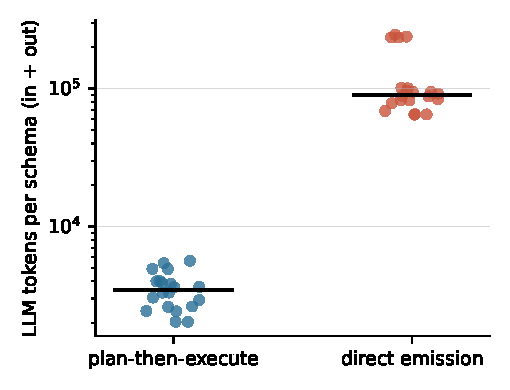
\includegraphics[width=0.5\textwidth]{figures/fig2_e1_tokens}
\caption{LLM tokens per schema cell (in + out, log scale; bars are medians): 3,472 for plan-then-execute versus 90,340 for direct emission.}
\label{fig:e1tokens}
\end{figure}

\begin{answer}{Answer to RQ2}
At 500 rows per table, plan-then-execute has no validity advantage over direct emission (medians 100\,\% and 98.7\,\%; paired difference $+0.004$, $p=0.85$), but it never violates a foreign key, CHECK or NOT NULL constraint, its misses are engine defects rather than data errors, it copies no fixture rows on any schema, and it costs one call and a median of 3,472 tokens against 14--45 calls and 90,340 tokens. Validity comes from the engine; recall is avoided by not letting the data pass through the model.
\end{answer}

\section{RQ3 (exploratory): provisioned data and LLM-generated tests}
\label{sec:rq3}
E2 is reported as an exploratory experiment, and the reason is stated first. With two runs per arm and 293 mutants, the paired exact test can detect a difference of roughly 6--12 mutants, which is the size of the baseline's own run-to-run variation (161 against 169 kills for Claude), and the 172 requirements contain few tests that cannot be written without existing data, which is where a fixture would be expected to matter. The experiment could therefore confirm a large effect and did not find one; it cannot rule out a small one. What it did identify is a mechanism on the yield side, and a single follow-up arm, designed after the main hypothesis had failed, that tests that mechanism against expectations written down before it ran. We present the kill-rate results, the yield mechanism and the follow-up in that order and with that weight.


\subsection{Usable yield and kill rate}
Table~\ref{tab:e2} and Fig.~\ref{fig:e2kills} give the aggregate results; Table~\ref{tab:e2pair} the paired statistics.

\begin{table}[t]
\centering\footnotesize\setlength{\tabcolsep}{4pt}
\caption{E2: mutants killed (of 293) and usable yield (known-good units / emitted units) per arm, provider and run.}
\label{tab:e2}
\begin{tabular}{lcccc}
\toprule
Arm & Claude r1 & Claude r2 & GPT-4o r1 & GPT-4o r2 \\
\midrule
G (grounded RAITG) & 161 (88\,\%) & 169 (89\,\%) & 106 (52\,\%) & 109 (59\,\%) \\
G + SynthData functional fixture & 158 (85\,\%) & 167 (84\,\%) & 115 (53\,\%) & 109 (49\,\%) \\
G + functional + edge/neg.\ payloads & 170 (83\,\%) & 167 (85\,\%) & 106 (50\,\%) & 113 (48\,\%) \\
G + project's own fixture & 145 (87\,\%) & 167 (81\,\%) & 109 (51\,\%) & 102 (48\,\%) \\
G + functional fixture + state contract (E2c) & 160 (93\,\%) & --- & --- & --- \\
\bottomrule
\end{tabular}
\end{table}

\begin{table}[t]
\centering\footnotesize
\caption{E2 paired versus G, same provider and run: difference in mutants killed, McNemar exact $p$, Holm-adjusted $p$ over the twelve pre-planned tests, bootstrap 95\,\% CI. The E2c arm was tested afterwards and is reported unadjusted.}
\label{tab:e2pair}
\resizebox{\textwidth}{!}{%
\begin{tabular}{llrrrrrr}
\toprule
Provider & Arm & r1 $\Delta$ & $p$ & $p_{\text{Holm}}$ & CI & r2 $\Delta$ ($p$) & CI \\
\midrule
Claude & functional & $-3$ & 0.51 & 1.0 & $[-9,+3]$ & $-2$ (0.75) & $[-8,+4]$ \\
Claude & func + edge/neg & $+9$ & 0.022 & 0.25 & $[+2,+16]$ & $-2$ (0.73) & $[-7,+3]$ \\
Claude & project fixture & $-16$ & $<$0.001 & 0.005 & $[-25,-8]$ & $-2$ (0.82) & $[-11,+6]$ \\
Claude & func + state contract (E2c) & $-1$ & 1.0 & --- & $[-6,+3]$ & --- & --- \\
GPT-4o & functional & $+9$ & 0.19 & 1.0 & $[-2,+22]$ & $0$ (1.0) & $[-9,+11]$ \\
GPT-4o & func + edge/neg & $0$ & 1.0 & 1.0 & $[-12,+11]$ & $+4$ (0.57) & $[-6,+14]$ \\
GPT-4o & project fixture & $+3$ & 0.63 & 1.0 & $[-5,+11]$ & $-7$ (0.19) & $[-16,+1]$ \\
\bottomrule
\end{tabular}}
\end{table}

\begin{figure}[t]
\centering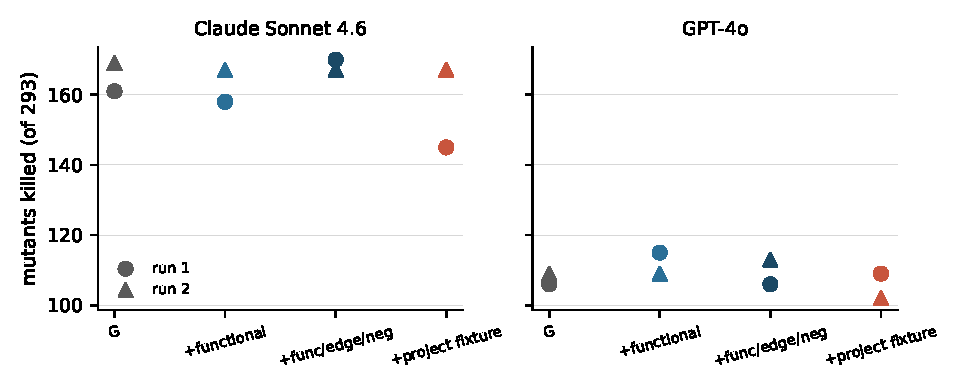
\includegraphics[width=\textwidth]{figures/fig4_e2_kills}
\caption{E2: mutants killed per arm (circles run 1, triangles run 2). No arm moves the kill rate reliably.}
\label{fig:e2kills}
\end{figure}


\paragraph{The advance hypothesis is rejected} A provisioned fixture does not raise usable yield. For Claude it lowers it, from 88--89\,\% to 83--85\,\%, and most on the task manager (known-good units 241 of 254 in G, 176 of 275 with the functional fixture). The failing units explain why: with 20 tasks pre-loaded, generated tests that create one task and assert a count of one, or that assume the row they created has id~1, fail on clean source, even though the prompt lists the pre-loaded rows and their ids. Provisioned rows conflict with the empty-database assumption the generator carries, and listing the rows does not remove the conflict.

\paragraph{Stating the contract restores the yield (E2c, one run, designed after the fact)} The G+D-state arm adds to the same functional block an explicit statement of what the pre-loaded rows imply for a test: ids $1..N$ are taken, a created row receives $N+1$, counts are relative to $N$. With the database state unchanged, usable yield returns to and slightly above the baseline: 1,207 of 1,294 units (93.3\,\%) against 87.9\,\% for G and 84.9\,\% for G+D-func, and on the task manager 271 of 281 (96.4\,\%) against 241 of 254 (94.9\,\%) and 176 of 275 (64.0\,\%). The generated tests read the contract: the failing patterns of G+D-func (assert a count of one; assume id~1) are replaced by tests that capture the id from the create response and assert relative counts or the presence of the row they created. The kill count is 160 against the baseline's 161 (paired difference $-1$; 2 arm-only and 3 baseline-only mutants; McNemar $p=1.0$; bootstrap CI $[-6,+3]$), with httpbin at $+1$, fastapi-restful and flaskr unchanged, and the task manager at 36 against 38 (32 with the functional block alone). All three expectations written down before the run hold; the arm is one run, added after the main hypothesis had failed, and is reported as a post-hoc observation rather than a tested finding. It is kept in the paper for one reason: it identifies the mechanism behind the yield loss of the planned arms (the generator's empty-database assumption) and names the specific contrast a powered follow-up should run, which the planned arms alone could not do. The block costs 16\,\% more input tokens than G (1.44M against 1.24M), about the same as the functional block alone. The yield loss of provisioning is therefore a fixture-contract problem that the prompt can solve; solving it does not change what the tests detect.

\paragraph{No arm reliably changes the kill rate} Of twelve paired comparisons, two are nominally significant and neither replicates. Claude with the boundary/negative payloads gains 9 mutants in run 1 ($p=0.022$; Holm-adjusted $p=0.25$), driven by fastapi-restful (16$\to$25), the validation-path mutants (409 on a duplicate squad number, 422 on an invalid payload) that the advance hypothesis named; in run 2 the baseline itself kills 25 on that service and the arm adds nothing. Claude with the project's fixture loses 16 in run 1 ($p<0.001$; Holm-adjusted $p=0.005$), a flaskr collapse (31$\to$15, with 113 of 163 units usable) that does not recur in run 2 (21). A 9-mutant change is 3 percentage points of the 293. GPT-4o's differences are within $\pm 9$ with 17--37 discordant mutants per comparison. The minimum difference the exact test can detect at these discordant counts is roughly 6--12 mutants, and the run-to-run variation of the baseline itself is of that size (161 versus 169 for Claude). httpbin, the service with no database and no block, moves by at most seven mutants (between $+1$ and $+7$ for Claude, between $-5$ and $+2$ for GPT-4o), inside the run-to-run band, as a control should. Two runs are not enough to separate a ten-mutant arm effect from run-to-run variation on this harness, and we report both runs rather than the favourable one.

\paragraph{Provider} GPT-4o is a different regime: about three tests per requirement (516 units per run against Claude's 1,300), half of them unusable, three to five times more repair passes, and 102--115 kills whatever the arm. The RAITG prompt was developed against Claude, so the two providers are not compared as equals; the null replicates on GPT-4o, which is all the second provider establishes.

\paragraph{Cost} The functional block adds 14\,\% input tokens per condition run (Claude 1.24M$\to$1.41M), the functional block with the state contract 16\,\% (1.44M), the full block 40\,\% (1.74M); output tokens change by less than 10\,\% and repair counts do not rise.

\begin{answer}{Answer to RQ3 (exploratory)}
At a sensitivity of 6--12 mutants, constraint-valid fixtures do not change the mutation kill rate of an existing LLM test generator (every Holm-adjusted $p=1.0$), and they lower the share of usable generated tests for Claude because the generated tests assume an empty database. One post-hoc arm shows that stating the database state in the prompt restores the yield (93\,\%) without changing the kill rate. A better-powered experiment, selecting requirements whose tests need existing data, is the follow-up this result motivates.
\end{answer}

\section{Discussion}
\label{sec:discussion}
\paragraph{What a team should do} Three practices follow. First, a team that asks a model for test data on a schema it did not design should assume that any realism it sees may be recall of published data, and treat the rows as fixtures of unknown provenance; the copy rates of Table~\ref{tab:copymodels} say that this is the common case on well-known schemas, for every model family, and more so for newer models. That matters for licensing as much as for validity: the Northwind rows a model emits are Microsoft's sample data, the HR rows are Oracle's. Second, if recall is unwanted, the route that avoids it is not a prompt but a design: let the model write the plan and an engine write the rows, which copies nothing, loads about as often, and costs a thirtieth of the tokens; the model's misses in direct emission are foreign-key and uniqueness violations that grow with schema difficulty, whereas the engine's misses are defects that can be fixed once. Third, if the purpose of the fixture is to help an LLM test generator, the fixture alone does not help and can hurt the yield; the generator needs to be told what state the database is in, and a provisioning tool should emit that state contract together with the rows.

\paragraph{What a researcher should do} An evaluation of LLM-generated data on a public schema needs a copy rate against the data that ships with the schema, computed against every edition of that data, because a revised fixture hides recall of the earlier one (Section~\ref{sec:editions}); and it needs a control that removes the cues by which the model recognises the schema, used as a lower bound, since a domain description alone identified Northwind for one model. The strongest control we can see is a schema that did not exist at the model's training cut-off, with data written for it; short of that, renaming identifiers, rewriting the business case and perturbing declared value lists together, and reporting the copy rate under each. The same applies to the schemas of the search-based test-data literature when a language model is added to them, and to any benchmark of LLM realism that scores against a public reference.

\paragraph{What the exploratory null means} E2's null is not that test data does not matter. The generated tests failed on provisioned data for a reason the study identified, and a one-paragraph change to the prompt removed the failure. The null is narrower and weaker than a tested finding: given a generator that already writes valid requests and assertions from the requirement text, supplying valid rows for it to read did not change which mutants its tests kill, at a sensitivity of six to twelve mutants out of 293 and on requirements that rarely need existing data. An experiment that selects for such requirements is the natural follow-up.

\section{Threats to validity}
\label{sec:threats}
\paragraph{Construct} Validity is measured as acceptance by PostgreSQL with declared constraints; undeclared business rules (an order line for a discontinued product) are invisible to it, and the human schemas declare almost no CHECK constraints, so the constraint surface is dominated by keys and nullability. The overlap metrics are column-wise and blind to cross-column coherence (a player whose position and abbreviation disagree, as SynthData's E2 fixtures do); the fixture arms in E2 test provisioning, not realism, and the project-fixture arm is the realism control. On free-text columns a low distance can only be achieved by knowing the data, which is why the metric family is named overlap rather than fidelity and why declared-domain and free-text columns are reported separately. The copy rate is computed against the fixture that ships today, and Section~\ref{sec:editions} shows that this is a lower bound whenever the fixture has been revised; we checked the editions of Oracle HR because its revision is documented, and have not checked the other seven. In E2, a kill is a failing or crashing unit; script-style units bypass pytest's per-test timeout, which is why the pre-screen exists.
\paragraph{Internal} The direct arm is the most favourable naive design we could build (parent keys shown, chunked, resumable); a weaker one would only widen the gap. The 500-row cap favours direct emission (Section~\ref{sec:method}). The renamed business cases keep their domain descriptions, and for Northwind the description identifies the dataset (Section~\ref{sec:copy}); E1b is therefore a lower bound on memorisation, and the copy rate is the measurement that does not depend on the control. Temperature 0 is not determinism: the same prompt produced plans that parsed and plans that did not, and run-to-run differences of ten mutants. The harness hardening in E2 was applied uniformly after discovery, and both scorings of the Claude baseline are on record. The E2 fixture's flaskr passwords are stored with a low PBKDF2 iteration count for timing reasons; login semantics are unchanged.
\paragraph{Conclusion} E1 has 20 cells over five schemas and E1b ten pairs; cells sharing a schema are not independent, the schema-level test ($n=5$) is reported alongside, and the renamed-versus-original copy-rate contrast is not significant ($p=0.30$), which is why the paper's claim rests on the copy rates themselves and not on the control. E1c adds 30 cells with one run each and no planned contrast, and is reported descriptively; the one repeated cell shows that the newest commercial models, which ran at their defaults rather than at temperature 0, vary between runs by more than the E1 models did. E2's two runs give a minimum detectable effect of 6--12 mutants, the size of the baseline's own run-to-run variation, and it is reported as exploratory. Twelve E2 tests are Holm-corrected; the E2c arm is a single run added afterwards, tested against expectations written before it ran, and reported unadjusted.
\paragraph{Reproducibility} The commercial models are versioned by the provider; the exact identifiers, dates and settings are in Section~\ref{sec:reporting} and every raw response is archived, so the analysis is reproducible from the artifact while the generation step is reproducible only as long as the providers serve those versions. The open-weight model's weights are public, but it was served through a router that used several hosts, each recorded per call; a replication on a single pinned host is the stricter form. Open weights do not open the training data either: Qwen3's pre-training corpus is described in its technical report only in aggregate and is not released, so for this model, as for the commercial ones, whether the fixtures were in the corpus cannot be checked by inspection, and the copy rate is the measurement that does not need the corpus. Two E1c models could not be run at temperature 0 and one reasons by default; the settings are logged per call. Temperature 0 is one control among several, not a guarantee (Section~\ref{sec:reporting}).
\paragraph{External} Eight schemas, five models, 500 rows per table; four services and two providers in E2. The eight schemas are the public sample databases a model is most likely to have read, which is the population the question is about, and not a sample of the schemas a team works on, where there is nothing to recall and the copy rate is zero by construction. Memorisation is only partly controlled: renaming removes lexical cues, not structural or domain ones (Sections~\ref{sec:e1b} and~\ref{sec:copy}). The copy rate counts exact and near-exact rows; a fixture row can also be reproduced with one value changed, which the near-match threshold of 0.9 catches only for short rows, and many valid rows exist for any schema, so similarity alone does not prove copying~\cite{riddell2024contamination}. The Faker and plan floors at zero, and the two schemas with nothing to recall at zero for every model, are what make the direct arm's rates interpretable. GPT-4o's low unit yield confounds the provider comparison in E2, and the E2 baseline is asymmetric (published Claude logs, fresh GPT-4o runs).
\paragraph{Conflict of interest} The tool is the author's, and the study uses it as the instrument for the plan arm. The mitigations are identical inputs and scoring for every arm, a version frozen before the first measured run, an independent no-LLM and a Faker baseline, published defects, and a released artifact that regenerates every number. The paper's central claim, that LLM-emitted test data on public schemas is recalled, does not depend on the tool at all, since it is measured on the direct arm against the shipped fixtures; the tool's own result is that its plans load no more often than emitted rows at 500 rows per table and that its misses are its defects, which does not favour it.

\section{Related work}
\label{sec:related}

\paragraph{LLMs as test-data generators} Baudry et al.~\cite{baudry2024generators} asked LLMs either to emit test data directly or to write test-data generator code, across languages and cultural contexts, and evaluated domain adequacy and executability; their generator-writing mode is the nearest precedent for plan-then-execute, and their evaluation did not check relational constraints or compare against human fixtures. Kannan et al.~\cite{kannan2025sqltestdata} generated test data for complex SQL schemas with an LLM in a privacy-restricted industrial setting and judged structural and semantic validity with schema checks and an LLM-as-a-judge; our scorer replaces the judge with the database. Neither study controlled for the possibility that the model had seen the data. Deep generative models for tabular data, from conditional GANs~\cite{xu2019ctgan} to fine-tuned language models that serialise rows as text~\cite{borisov2023great} and to relational extensions that generate child tables conditioned on parents~\cite{solatorio2023realtabformer}, target distributional fidelity for machine-learning use and check copying with a distance-to-closest-record test against the rows the model was fine-tuned on. That test asks whether a generator copies its training table; our question is whether a foundation model copies a table it was never fine-tuned on but has read many times, which the distance-to-closest-record test cannot see and the renamed-schema control and copy rate can. Our consumer is a test, so hard constraints are the primary requirement. And our data is requested for a public schema rather than sampled from a private table, which is what raises the recall question.

\paragraph{Test data for database applications} AGENDA~\cite{chays2004agenda} populated databases from schema constraints and user-supplied value sets; later work generated databases to satisfy declarative constraints and cardinality targets~\cite{arasu2011declarative}, produced realistic values at scale for benchmarking~\cite{bruno2005flexible,houkjaer2006simple}, derived inputs from the queries a program issues~\cite{emmi2007dynamic}, and defined coverage criteria over SQL predicates~\cite{tuya2010full}. Search-based generation of test data for a schema's integrity constraints~\cite{kapfhammer2013search,mcminn2015effectiveness} is the closest ancestor of the engine studied here. McMinn et al.\ use acceptance or rejection of INSERT statements by a real DBMS as the oracle and mutation analysis of the schema as the measure of test strength, over 32 schemas and three DBMSs; that is the methodological template our scorer and E2 follow. EvoSQL~\cite{castelein2018evosql} generates data to cover the predicates of the SQL queries a program issues, which is the coverage-oriented sense of ``useful test data'' that E2 tests from the other side. SynthData's \texttt{negative} profile is a generator-vocabulary rendering of the constraint-coverage idea, and our scorer is the oracle those works rely on. Several of the schemas in that literature (Dell DVD Store, the PostgreSQL sample databases) are the same public schemas an LLM has read, which is why any reuse of that benchmark with a language model needs the control introduced here. None of this literature considered a language model as the author of the generator.

\paragraph{Memorisation and contamination} That language models reproduce training data verbatim is established~\cite{carlini2021extracting}. The rate at which they do so grows with model size, with the number of times a sequence is duplicated in the training data, and with the length of the prompt that cues it~\cite{carlini2023quantifying}; the sample databases studied here are duplicated across two decades of tutorials, which is the condition under which that rate is highest. Benchmark contamination is a recognised problem in natural-language evaluation~\cite{magar2022contamination,sainz2023contamination,golchin2024timetravel}. For code benchmarks, Riddell et al.~\cite{riddell2024contamination} measured it with exact and edit-distance matching against the training corpora and re-evaluated on the uncontaminated subset. Our copy rate applies the same matching to relational rows, and our renamed-schema control plays the role of their unseen subset, since the providers' training corpora are closed. Golchin and Surdeanu~\cite{golchin2024timetravel} detect contamination by contrasting a prompt that names the dataset with one that does not; the original and renamed schemas are that contrast for relational fixtures. For code, ReCode~\cite{wang2023recode} evaluates generation models under semantics-preserving perturbations, including identifier renaming; the renamed-schema control is the same idea applied to relational fixtures, whose value is precisely that they are public and long-lived, so held-out data is not available. Its result---an overlap with the fixtures that disappears under renaming while validity does not move---is the relational counterpart of the contamination effects reported for text benchmarks, and we are not aware of a prior measurement of it for LLM-generated test data.

\paragraph{LLM-generated tests and their execution} LLM unit-test generation has been evaluated on coverage and correctness~\cite{schafer2024testpilot,siddiq2024junit,yuan2024chattester,chen2024chatunitest}, at scale across models and prompt designs~\cite{ouedraogo2026emse,walczak2026jss}, from requirements text rather than code~\cite{alagarsamy2025jss}, with mutants as the measure of test strength and as prompt feedback~\cite{dakhel2024mutap}, compared with search-based generation~\cite{tang2024chatgptsbst} and combined with it~\cite{lemieux2023codamosa}; surveys~\cite{wang2024survey} catalogue the design space. Those studies treat contamination in three ways or not at all: an edit-distance check of generated tests against the project's existing tests~\cite{schafer2024testpilot,yuan2024chattester}, a split of subjects into projects seen and unseen at the model's training cut-off~\cite{chen2024chatunitest}, and silence~\cite{dakhel2024mutap}. Our design combines the first two, as a copy rate against the shipped data and a renamed-schema control, and adds non-LLM floors. Where these studies evaluate against mutated programs they inherit mutation analysis and its caveats about mutant validity~\cite{just2014mutants,papadakis2019mutation}; E2 reuses an existing, archived executable benchmark so that the only variable is the data block. Two findings anticipate ours: generated tests often fail for environmental reasons, such as wrong fixtures and assumptions about state~\cite{schafer2024testpilot,yuan2024chattester}, and the test-pattern literature distinguishes fresh fixtures built by each test from shared or prebuilt fixtures that tests must respect~\cite{meszaros2007xunit}. LLM-generated tests, in our data, behave as if every fixture were fresh.

\paragraph{Faker} The de facto tool for test data in Python is Faker~\cite{faker}, which produces plausible scalar values with no notion of a schema; our Faker arm is that default applied per table, and its foreign-key failures on four of five schemas quantify what a relational engine adds before any LLM is involved.

\section{Conclusion}
\label{sec:conclusion}
The realism that LLM-emitted test data shows on well-known schemas is, to a large and measurable extent, recall of the published fixtures. Five models from three vendors, including an open-weight one, reproduce the rows of Northwind, Chinook and Pagila verbatim, at rates from a few per cent to three quarters of the emitted rows, and the newer model of each vendor reproduces more than its predecessor. The recall can be invisible to a measurement against the fixture that ships today: Oracle rewrote its HR data in 2021, and the models recite the earlier editions, one of them in full. A renamed-schema control removes the distributional overlap, which is consistent with recall and not with a harder schema, but does not remove copying cued by a domain description, so it is a lower bound and not a substitute for the copy rate. Letting the model write a plan and an engine write the rows copies nothing, loads about as often at 500 rows per table, and costs a thirtieth of the tokens. An exploratory downstream experiment found no reliable change in what an LLM test generator detects when given valid fixtures, at a sensitivity of six to twelve mutants, and identified why the fixtures lowered its usable yield. Evaluations of LLM data generation on public schemas should report a copy rate against every edition of the shipped data, and should treat a control that renames the schema as the floor of what the model remembers, not the ceiling.

\section*{Declarations}
\paragraph{Funding} The author received no funding for this work; the API costs of the experiments were paid by the author.

\paragraph{Competing interests} The author is the developer of SynthData, the plan-then-execute engine used as an instrument in this study; Section~\ref{sec:threats} states the mitigations. The author has no other competing interests.

\paragraph{Ethics approval and consent} Not applicable; the study involves no human participants and no personal data. The fixtures are the sample data published with open-source database schemas.

\paragraph{Data and code availability}
\label{sec:data}
The complete artifact (pinned subjects with checksums, canonical and renamed DDLs with rename maps, frozen business cases, row targets, the E2 DDLs, cases, fixtures and prompt blocks, every arm's output with per-call tokens and latency, every score and metric file, the copy-rate scripts and their per-table results for E1, E1b and E1c, the E1c arm outputs with per-call logs including the serving host and sampling settings, the Postgres ports of the three E1c schemas and the three editions of the Oracle HR fixture, the per-mutant kill vectors, known-good lists and pre-screen records of E2, the scoring harness, the cell-table builder and the scripts that regenerate every table, figure and statistic in this paper) is archived on Zenodo as \texttt{paperH-artifact}, version 1.2.1, DOI \href{https://doi.org/10.5281/zenodo.23173140}{10.5281/zenodo.23173140} (version 1.1.0, DOI \href{https://doi.org/10.5281/zenodo.22939052}{10.5281/zenodo.22939052}, holds E1, E1b and E2; versions 1.2.x add E1c and the model-identity check) and mirrored at \href{https://github.com/javvadivijayprasad/llm-testdata-memorisation}{github.com/javvadivijayprasad/llm-testdata-memorisation} (tags \texttt{v1.1.0} and \texttt{v1.2.1}, the same files). SynthData~1.2.2 is published on npm; its file checksums are in the artifact.

\paragraph{Author contribution} Vijay Prasad Javvadi is the sole author and carried out the conceptualisation, design, implementation, data collection, analysis and writing.

\paragraph{Use of generative AI} Two groups of LLM calls appear in this paper. The experimental subjects (the models and API settings in Section~\ref{sec:reporting}) are described in the paper and every call is logged in the artifact. Separately, Claude (Anthropic) was used as a coding and drafting assistant under the author's direction for the harness and analysis scripts and for copy-editing; the author ran all code, checked every reported number against the result files, and takes full responsibility for the content.

\appendix
\section{E2 harness corrections}
\label{app:harness}
Two harness issues surfaced during scoring and were fixed before any number was final; both are recorded because the second changes a baseline. First, the fixture's password hashing (werkzeug's default 260k PBKDF2 rounds, re-run before every test and on every \texttt{init\_db()} call) pushed the flaskr suite past the scorer's 90-second limit, which the RAITG protocol counts as a kill. Hashes are therefore memoised with a low iteration count; logins are unaffected, since the verifier reads the method from the stored hash. Second, one GPT-4o flaskr unit calls the application's \texttt{init\_db\_command()} at module level. The resulting \texttt{SystemExit} inside pytest's collection aborted every pytest process for that service. The original group-level known-good filter could not attribute the failure to a unit and kept all 130, and the scorer then saw the same exit status on the baseline and on every mutant, that is, zero kills. The E2 harness therefore adds a per-unit pre-screen before the known-good filter: each unit runs alone under a 30-second wall cap (the limit the RAITG protocol already applies per test function, which pytest's timeout cannot apply to module-level code), and units that cannot pass alone are excluded and recorded. The pre-screen removes units; it cannot add kills. Every arm, including the baseline for both providers, was re-scored under this one harness before any comparison was made. The Claude baseline logs re-scored under it give 161 and 169 kills against the archived 160 and 159; the difference is three fastapi-restful units that pass only after an earlier unit has warmed the service's ten-minute response cache, order-dependent units that the stricter filter removes. No E2 chunk contains a timeout-based kill.

\bibliographystyle{elsarticle-num}
\bibliography{references}
\end{document}
